\subsection {Problema de Ruteo de Vehículos (VRP)}

\subsubsection {Definición y Características}
El Problema de Ruteo de Vehiculos (VRP por las siglas de su nombre en Ingles "Vehicle Routing Problem") nace como una generalización del Traveling Salesman Problem (TSP) que según \cite{[DANTZIG-RAMSER]} se enuncia de la siguiente forma:“Existe una flota determinada de vehículos los cuales tienen una capacidad limitada que parten de un mismo punto inicial y deben satisfacer la demanda de determinados puntos".\\
En la actualidad, el VRP ha alcanzado una gran cantidad de variantes, presentando distinta capacidad y múltiples depósitos.
Como se puede ver en la imagen  \ref{fig:Ejemplo-VRP}, se tiene un ejemplo de VRP, como se puede apreciar es parecido al TSP, solo que una misma ruta puede fragmentarse en varias para cubrir mas espacio en poco tiempo.

    \begin{figure}[hbtp]
        \centering
            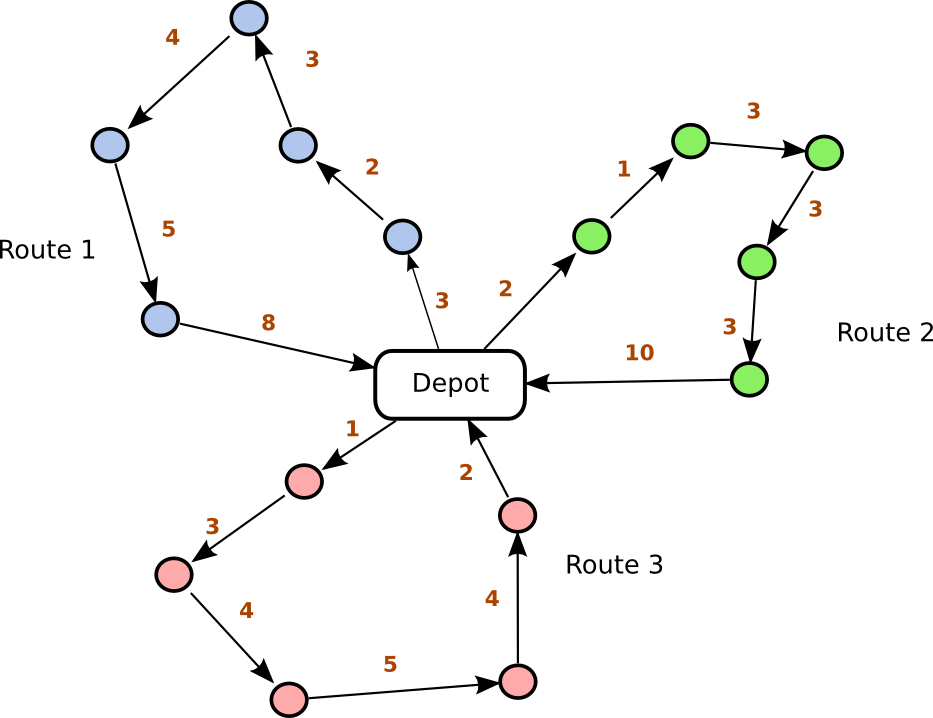
\includegraphics[width=0.6\textwidth]{MarcoTeorico/Imagenes/vrp_Ejemplo.png}
            \caption{Ejemplo de VRP.}                       
            \label{fig:Ejemplo-VRP}
    \end{figure} 

\subsubsection {Variantes del VRP}
Según \cite{[GOLDEN-ASSAD]}, las variantes del VRP son:
\begin{itemize}
\item \textbf{Vehicle Routing Problem With Time Windows (VRPTW) : }Al cliente se le asocia  un intervalo de tiempo en donde se encontrará disponible a recibir los productos. 
\item \textbf{Capacited Vehicle Routing Problem (CVRP) : } Es el más general y básicamente consiste en que existen vehículos con capacidad limitada y constante, los cuales son los encargados de suplir la demanda de los clientes.
\item \textbf{Multi-Depot Vehicle Routing Problem (MDVRP) : }Tiene múltiples depósitos, donde cada uno de estos depósitos tiene una flota de vehículos independiente.
\item \textbf{Periodic Vehicle Routing Problem (PVRP) : }Contempla un tiempo de operación donde los clientes deben ser visitados una vez. 
\item \textbf{Split Delivery Vehicle Routing Problem (SDVRP) : }Los vehículos pueden atender a más de un cliente siempre y cuando exista una reducción del costo total.
\item \textbf{Stochastic Vehicle Routing Problem (SVRP) : } Da la posibilidad que uno o varios componentes sean de carácter aleatorio.
\item \textbf{Pick-Up and Delivery Vehicle Routing Problem (VRPPD) : }Es aquel en donde cabe la posibilidad de que los clientes puedan devolver material.
\item \textbf{Mix Fleet Vehicle Routing Problem (MFVRP) : }Este modelo supone vehículos con capacidades heterogéneas, por lo que un camión más grande podrá recorrer mayores distancias o suplir mayores requerimientos de las distintas ciudades. 
\end{itemize}

\subsubsection {Modelado Matemático }

\subsubsection {Aplicaciones}
\textbf{Reprogramación del transporte forestal}\\
(Obtenido de \cite{[ARANEDA]})\\
El transporte terrestre, en particular el de camiones, es el más empleado en el sector forestal, dada su alta versatilidad y variedad de medios para acceder a los puntos de origen de materia prima (bosques) y llegar a los centros de proceso o destino (plantas de proceso).\\
En Chile, las empresas forestales (empresas mandantes) subcontratan el servicio de transporte terrestre a diferentes empresas de servicios llamadas EMSEFOR. Esta programación es efectuada utilizando un software desarrollado para ese fin, llamado “asignador de camiones” (ASICAM).\\
El problema consiste en lograr mejores propuestas de asignación a partir de la asignación lograda con ASICAM. 
Para resolverlo se utiliza un algoritmo de optimización Multiobjetivo para el transporte forestal basado en la Metaheurística de colonias de hormigas. Este algoritmo reprograma la agenda diaria de camiones-rutas, el cual asigna camiones a los trabajos de transporte a realizar en las faenas forestales.\\
La validación del algoritmo propuesto se logra resolviendo un problema real en el cual se plantearon dos objetivos, esto es, reducir el número de camiones programados y disminuir el tiempo total recorrido por
los camiones en las rutas asignadas por ese sistema.\\
Estos objetivos provocan un impacto directo en los costos involucrados en el proceso de transporte forestal.

\textbf{Reprogramación del transporteforestal}\\
(Obtenido de \cite{[PEMBERTHY]})\\
Consiste en realizar la programación de operaciones de transporte internacional entre dos países, Colombia y Venezuela, para un horizonte de tiempo con múltiples variantes; entre ellas podemos resaltar: una flota heterogénea de vehículos y tráileres, múltiples depots (clientes), restricciones de ventanas de tiempo en los depots, diversas modalidades de servicio, entre otras. \\
Este trabajo se enfoca en dar solución a un problema real de planificación de transportes o ruteo de vehículos, definido gracias al aporte de una empresa colombiana del sector de servicios de transporte por carretera.\\
La solución se realizó a través de la implementación de la metaheurística Recocido Simulado (SA, Simulated Annealing), la cual se probó iniciando con soluciones factibles generadas por dos algoritmos heurísticos; el primero se basa en la heurística clásica conocida como el vecino más cercano y el segundo genera soluciones de forma aleatoria. \\
Los resultados del Recocido Simulado usando las soluciones generadas con el primer algoritmo, no mostraron una mejora frente a dicha solución inicial, contrario a lo hallado con el uso de las soluciones del segundo método, donde se alcanzó hasta cerca de un 50 \%  de mejora.\\

\textbf{Asignación óptima de ruta para las clínicas móviles}\\
(Obtenido de \cite{[CONTARDO]})\\
Se presenta el problema de ruteo de vehículos para la asignación de un solo vehículo (SVRAP) y se postula un algoritmo de búsqueda tabú para su solución.\\
SVRAP es el problema de decidir una ruta para un sólo vehículo (a partir de un lugar determinado y que termina en una ubicación dada) de tal manera que se visita un conjunto de clientes. Sin embargo, en contraste con el habitual problema de ruteo de vehículos, no todos los clientes deben ser visitados. \\
Los clientes no visitados por el vehículo o bien se puede asignar a un cliente que esté en la ruta del vehículo, o pueden ser aislados. El objetivo es reducir al mínimo una suma ponderada de los costos del ruteo, asignación y el aislamiento. 

%\subsubsection {Técnicas del Solución }


